\documentclass[UTF8]{ctexart}

\usepackage{amsmath}
\usepackage{subfigure}
\usepackage{hyperref}

\usepackage[graphicx]{realboxes}


\title{Image Caption 学习笔记 Week 3}
\author{高崧淇}
\date{\today}

\begin{document}

    \maketitle
    \tableofcontents


    \section{论文阅读——利用人类反馈}

    \subsection{简介}

    \subsection{Training language models to follow instructions with human feedback~\cite{ref_igpt}}
    以往,GPT-3 也很可能产生不真实、有害或反映不良情绪的输出。
    这在一定程度上是因为,在互联网文本的大数据集上,训练 GPT-3 来完成下一个单词的预测,并非是安全地执行用户想要的语言任务。
    换句话说,这些模型与其用户可能实际上并不一致。

    为了让模型更安全、更有用、更一致,OpenAI 使用了一种称为从人类反馈中强化学习(RLHF,Reinforcement Learning from Human Feedback)的技术。
    根据客户向 API 提交的反馈,OpenAI 对模型的多个输出进行排序。然后,OpenAI 使用这些数据来微调 GPT-3。
    由此产生的 InstructGPT 模型,在遵循指令方面,远比 GPT-3 要好得多。而且,它们也较少的凭空捏造事实,有害输出的产生呈现小幅下降趋势。

    \paragraph{RLHF}
    \begin{figure}
        \centering
        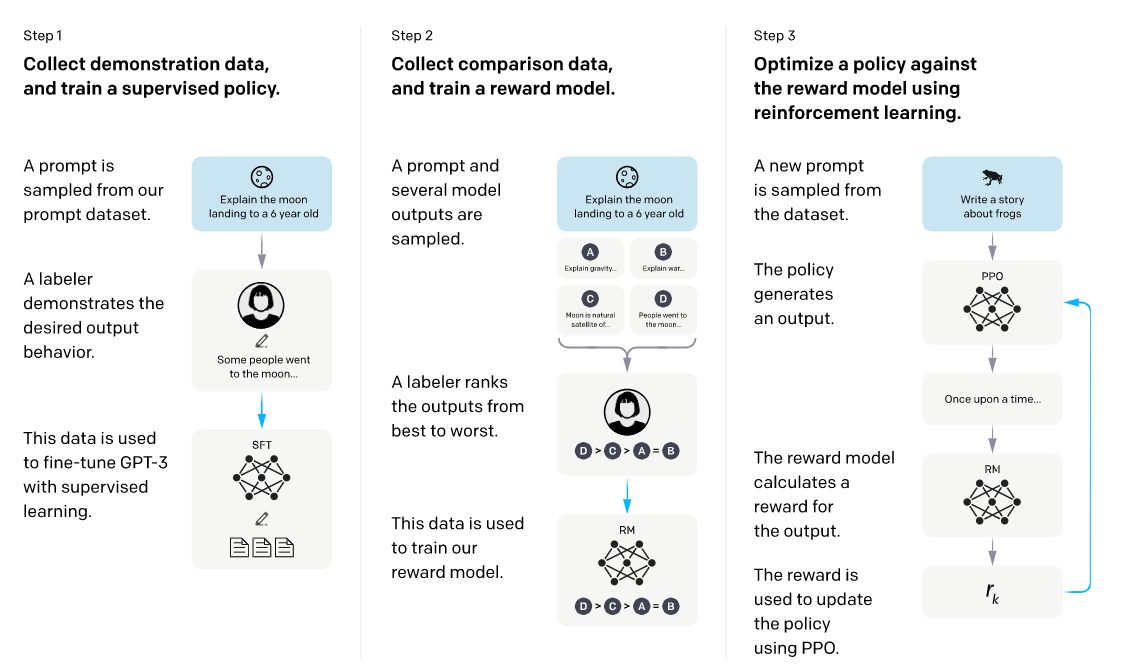
\includegraphics[width=\textwidth]{rm}
        \caption{OpenAI的方法}
        \label{fig:rm}
    \end{figure}

    OpenAI的RLHF总共分三步~\ref{fig:rm}:
    \begin{itemize}
        \item[$1.$] 找一些人写下示范答案,来微调GPT-3模型,训练监督模型baseline。
        \item[$2.$] 收集某个问题的几组不同输出数据,由人类对几组答案进行排序,在此数据集上训练奖励模型。
        \item[$3.$] 使用RM作为奖励函数,近端策略优化(PPO)算法微调GPT-3策略,以强化学习方法最大化奖励。
    \end{itemize}

    这种方法存在一个局限性在于它引入了“对齐问题”,因为模型仅根据对齐客户的NLP任务,那么可能会在学术NLP任务上的表现更糟。
    OpenAI发现了一个简单的算法更改,可以最大限度地减少该问题:在强化学习微调期间,混合用于训练GPT-3原始数据的一小部分,
    并使用正态似然对最大化(normal log likelihood maximization)来训练这些数据。

    \subsection{Learning to summarize from human feedback~\cite{ref_human}}
    从人工反馈中学写摘要
    \paragraph{Seq2Seq架构的问题和解决方案}

    \subparagraph{Exposure bias}
    Seq2Seq模型在训练和推理时,方式有很明显的不同。训练阶段模型根据GT来生成(teacher forcing),
    推理时不知道GT,当前步依赖于前一步(一步错步步错),这会带来在这两阶段非常大的数据分布的差异。
    一直以来有Seq2Seq领域有很多的研究在处理这个注明的Exposure bias问题。

    \subparagraph{Metrics}
    一般文本生成任务常用BLEU或者ROUGE做metrics。大致上就是看看在生成句子和参考句子之间有多少n-gram的overlap。
    传统的Seq2Seq在metrics方面做得很差。首先,Cross Entropy作为损失函数,根本没有直接对metrics进行优化。
    这个问题常用的解决思路是利用强化学习,特别是policy gradient,它可以直接针对reward进行优化。
    在这里直接把reward定义为metrics就可以。另外,BLEU或者ROUGE属于比较粗糙的metrics。
    文本生成的结果可以千变万化,其实区区的n-gram重合能够描述的。
    我印象中曾有用生成句子和参考句子的embedding的cosine similairity来做metrics的研究,这就比BLEU这种土办法强了很多倍。

    当然了,最强的metrics其实只能由人类来产生。比如一个句子翻译的好不好,有相关经验的人一看便知。
    有一类做法是利用GAN里的discriminator来产生metircs:它产生的概率D(x)表示生成的句子和真实的结果有多相似。
    这里的相似可不是有多少的n-gram重合,而是数据分布上的相似。OpenAI的做法和GAN不一样,作者直接利用人的反馈作为label另外作了一个reward模型,
    这样,弱metrics的问题就解决了。

    解决方案
    其实强化学习可以同时兼顾以上的两个痛点。针对exposure bias,强化学习在训练的时候就可以避免填鸭式(teacher forcing)。
    以策略学习为例,



    \begin{thebibliography}{8}
        \bibitem{ref1}
        Kafle, Kushal, and Christopher Kanan.
        "Visual question answering: Datasets, algorithms, and future challenges."
        Computer Vision and Image Understanding 163 (2017): 3-20.

        \bibitem{ref_igpt}
        Long Ouyang et al. “Training language models to follow instructions with human feedback”  (2022).
        \bibitem{ref_human}
        Nisan Stiennon et al. “Learning to summarize from human feedback” neural information processing systems (2020): n. pag.
    \end{thebibliography}

\end{document}
